%%%% Paramétrage du TD %%%%
\def\xxauteur{\textsl{Xavier Pessoles}}

\def\xxnumchapitre{Chapitre 1 \vspace{.2cm}}
\def\xxchapitre{\hspace{.12cm} Stabilité des systèmes}

\def\xxcompetences{%
\textsl{%
\textbf{Savoirs et compétences :}\\
\vspace{-.4cm}
\begin{itemize}[label=\ding{112},font=\color{bleuxp}] 
%\item \textit{Mod3.C2 : } pôles dominants et réduction de l’ordre du modèle : principe, justification
%\item \textit{Res2.C4 : } stabilité des SLCI : définition entrée bornée -- sortie bornée (EB -- SB)	
%\item \textit{Res2.C5 : } stabilité des SLCI : équation caractéristique	
\item \textit{Res2.C6 : } stabilité des SLCI : position des pôles dans le plan complexe
\item \textit{Res2.C7 : } stabilité des SLCI : marges de stabilité (de gain et de phase)
\end{itemize}
}}


\def\xxfigures{
%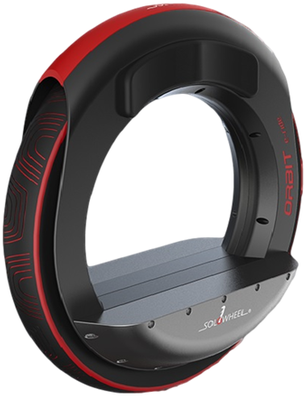
\includegraphics[width=3cm]{SoloWheel_Orbit}\\
%\textit{}
}%figues de la page de garde

\def\xxtitreexo{Activation}
\def\xxsourceexo{\hspace{.2cm} \footnotesize{Patrick Dupas, \url{http://patrick.dupas.chez-alice.fr/}.}}
\def\xxactivite{Activation\ifprof \\ Corrigé \else \fi}
%\def\xxauteur{\textsl{P. Dupas.}}

\input{\repRel/Style/pagegarde_TD}

\setlength{\columnseprule}{.1pt}
\pagestyle{fancy}
\thispagestyle{plain}


\vspace{4.5cm}

\def\columnseprulecolor{\color{bleuxp}}
\setlength{\columnseprule}{0.4pt} 

%%%%%%%%%%%%%%%%%%%%%%%



\ifprof
\else
\begin{multicols}{2}
\fi

\subsection*{Exercice 1 -- Réponse impulsionnelle (entrée Dirac)}
\setcounter{numques}{0}
\ifprof
\else
\begin{center}
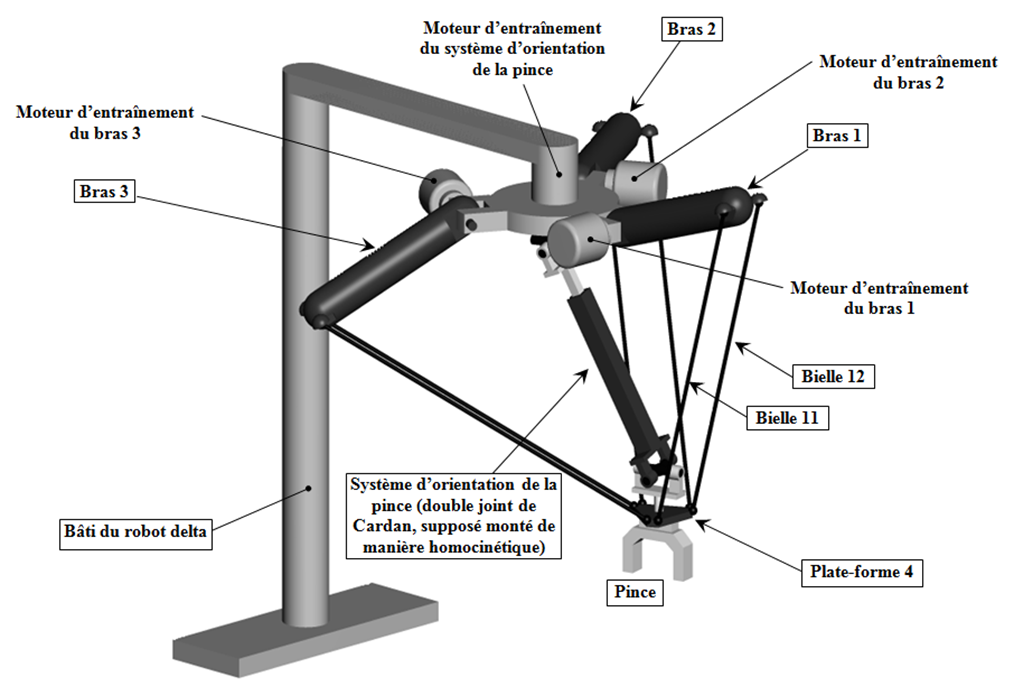
\includegraphics[width=\linewidth]{fig_01}
\end{center}
\fi
\question{Pour chaque cas déterminer si la réponse est celle d'un système stable, instable ou juste (quasi) stable.}

\subsection*{Exercice 2 -- Pôles de la FTBF}
\setcounter{numques}{0}
\ifprof
\else
On donne les pôles des FTBF de plusieurs systèmes :
\begin{multicols}{2}
\begin{enumerate}
\item $-1$, $-2$;
\item $-3$, $-2$, $0$;
\item $-2+j$, $-2-j$, $2j$, $-2j$;
\item $-2+3j$, $-2-3j$, $-2$;
\item $-j$, $j$, $-1$, $1$;
\item $-1$, $+1$;
\item $-1+j$, $-1-j$;
\item $2$, $-1$, $-3$;
\item $-6$, $-4$, $7$.
\end{enumerate}
\end{multicols}
\fi
\question{Pour chaque cas déterminer si la réponse est celle d'un système stable, instable ou juste  (quasi) stable.}





\subsection*{Exercice 3 -- Applications du critère du Revers}
\setcounter{numques}{0}

\question{On donne ci-dessous les lieux de transferts de plusieurs {\text{FTBO}}. Déterminer, à l'aide du critère du Revers si les systèmes sont stables en BF.}

\question{Pour les systèmes stables déterminer les marges de gain et de phase.}

%
%
%\begin{center}
%\includegraphics[width=\linewidth]{OLD/fig_02}
%\end{center}
%
%\begin{center}
%\includegraphics[width=\linewidth]{OLD/fig_03}
%\end{center}
\ifprof
%\begin{center}
%\includegraphics[width=.45\linewidth]{OLD/fig_04}
%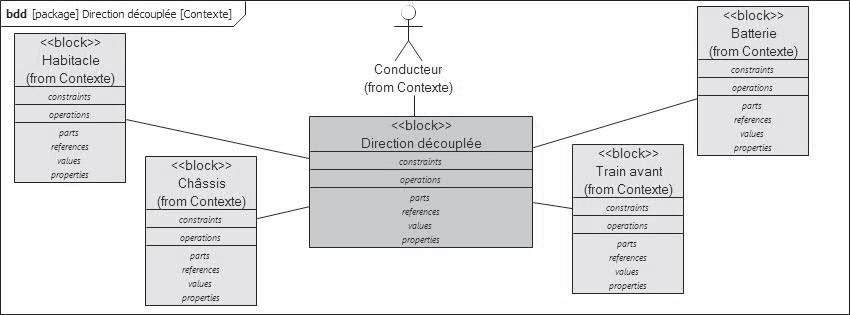
\includegraphics[width=.45\linewidth]{OLD/fig_05}
%\end{center}
\else
\begin{center}
\includegraphics[width=\linewidth]{OLD/fig_04}
\end{center}

\begin{center}
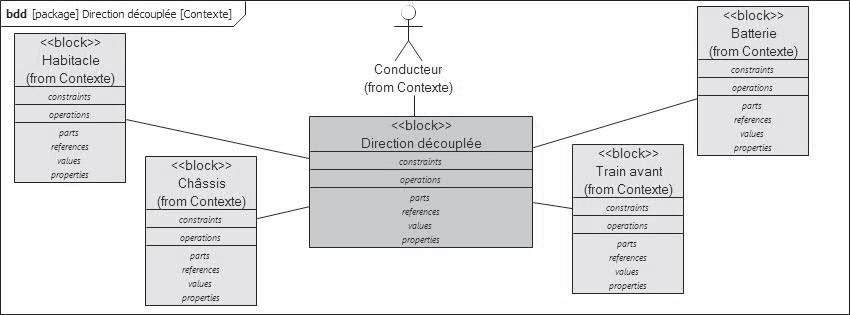
\includegraphics[width=\linewidth]{OLD/fig_05}
\end{center}
\fi


%\newpage

\subsection*{Exercice 4 -- Étude de la stabilité}
\setcounter{numques}{0}



\ifprof
\else

\begin{obj}
\begin{itemize}
\item Caractériser la stabilité d'un système à partir de la {\text{FTBO}}.
\item La marge de gain est supérieure à $\SI{10}{dB}$ et que la marge de phase est supérieure à \SI{45}{\degres}.
\end{itemize}

\end{obj}


On donne le schéma bloc suivant :

\begin{center}
\includegraphics[width=.6\linewidth]{fig_02}
\end{center}

\fi

On a $K=1$, $\tau = 0,1$ et $G=20$. 
%
%\question{Justifier la forme du schéma-blocs retenu pour modéliser la {\text{FTBO}} qui sera notée $H(p)$.}
%\ifprof
%\begin{corrige}~\\
%On a $H(p)=\dfrac{S(p)}{E(p)}
%=\dfrac{\dfrac{KG}{\left(1+\tau p\right)p}}{1+\dfrac{KG}{\left(1+\tau p\right)p}}
%=\dfrac{1}{\dfrac{\tau}{KG} p^2+\dfrac{p}{KG}+1}$.
%
%Ainsi, $H(p)$ est un système du second ordre avec un gain unitaire, comme la fonction identifiée dans les premières questions. 
%\end{corrige}
%\else
%\fi
%
%On considère le correcteur proportionnel $K=1$. 
%\question{Déterminer les valeurs de $G$ et de $\tau$ et en déduire $H(p)$.}
%\ifprof
%\begin{corrige}~\\
%On a :
%$\dfrac{1}{\dfrac{\tau}{G} p^2+\dfrac{p}{G}+1}
%= \dfrac{1}{1+0,05p+0,005p^2}$. En conséquences, $G=20$ et $\tau/20=0,005 \Rightarrow \tau=\SI{0,1}{s}$ et ${\text{FTBO}}(p)=\dfrac{20}{(1+0,1p)p}$.
%
%\end{corrige}
%\else
%\fi

\question{Déterminer l'erreur statique et l'erreur de traînage.}

\ifprof
\begin{corrige}
Ici on a $\varepsilon(p)=\dfrac{E(p)}{1+{\text{FTBO}}(p)}$. 

Erreur statique (entrée échelon): $\varepsilon_s 
= \lim\limits_{t\to +\infty} \varepsilon(t)
= \lim\limits_{p\to 0} p\varepsilon(p)
= \lim\limits_{p\to 0} p \dfrac{1}{p}\dfrac{1}{1+\dfrac{20}{(1+0,1p)p}}=0$

Erreur trainage (entrée rampe): $\varepsilon_t
= \lim\limits_{t\to +\infty} \varepsilon(t)
= \lim\limits_{p\to 0} p\varepsilon(p)
= \lim\limits_{p\to 0} p \dfrac{1}{p^2}\dfrac{1}{1+\dfrac{20}{(1+0,1p)p}}=1/20$
\end{corrige}
\else
\fi


\question{Effectuer les tracés des diagrammes de Bode de la {\text{FTBO}}.}
\ifprof
\begin{corrige}~\\


\begin{center}
%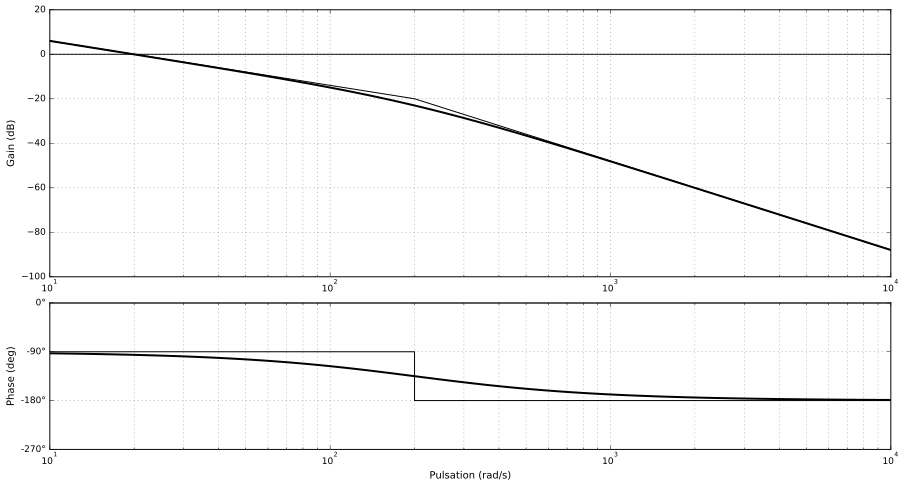
\includegraphics[width=\linewidth]{cor_01}
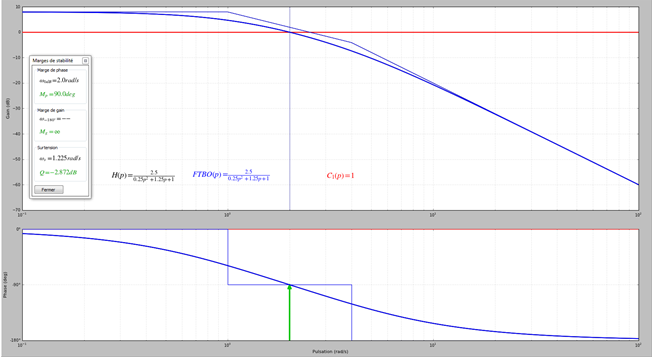
\includegraphics[width=.8\linewidth]{cor_03}
\end{center}
\end{corrige}
\else
\fi
%Le cahier des charges impose une marge de gain de $\SI{10}{dB}$ et une marge de phase de $
%\SI{45}{\degree}$.


\question{Déterminer graphiquement les marges de gains et de phase.}
\ifprof
\begin{corrige}~\\
\end{corrige}
\else
\fi

\question{Confirmer ces résultats par le calcul.}
\ifprof
\begin{corrige}~\\
La phase ne coupe jamais l'axe des abscisses. Ainsi, La marge de gain n'est pas définie (elle est infinie).
Pour déterminer la marge de phase analytiquement :
\begin{enumerate}
\item On cherche $\omega_c$ tel que $G_{\text{dB}}(\omega_c)=0$;
\item On calcule $\varphi(\omega_c)$;
\item La marge de phase est de $\varphi(\omega_c) -(-180)$.
\end{enumerate}

Cherchons $\omega_c$ tel que $G_{\text{dB}}(\omega_c)=0$. 
On a ${\text{FTBO}}(j\omega )
=\dfrac{20}{(1+0,1j\omega)j\omega}
=\dfrac{20}{j\omega-0,1\omega^2}$. 
$20\log |{\text{FTBO}}(j\omega )| 
= 20\log 20 - 20\log \sqrt{\omega^2+0,01\omega^4}
= 20\log 20 - 20\log \omega\sqrt{1+0,01\omega^2}$.

 $G_{\text{dB}}(\omega_c)=0 
\Leftrightarrow   20 =\omega_c\sqrt{1+0,01\omega_c^2} 
\Leftrightarrow   400 =\omega_c^2 \left(1+0,01\omega_c^2\right)$
On pose $x=\omega_c^2$ et on a :
$400 =x \left(1+0,01x\right)\Leftrightarrow x^2+100x-40000=0$. 
On a donc $\Delta = 412,3^2$ et $x_{1,2}=\dfrac{-100\pm412,3}{2}$ on conserve la racine positive et  $x_1=156,15$ et $\omega_c=\SI{12,5}{rad.s^{-1}}$.

$\varphi(\omega_c)=\arg(20)-90 -\arg\left(1+0,1j\omega_c \right)
=0- 90 -\arctan\left( 0,1\omega_c \right)
=0-90-51,34=-141,34\degres$.

La marge de phase est donc de 38,66\degres.
\end{corrige}
\else
\fi

\question{Conclure par rapport au cahier des charges.}
\ifprof
\begin{corrige}
Le système ne sera pas stable vis-à-vis du cahier des charges.
\end{corrige}
\else
\fi

\ifprof
%\begin{corrige}
%\end{corrige}

Pour $\tau  = 0,005$


\begin{center}
%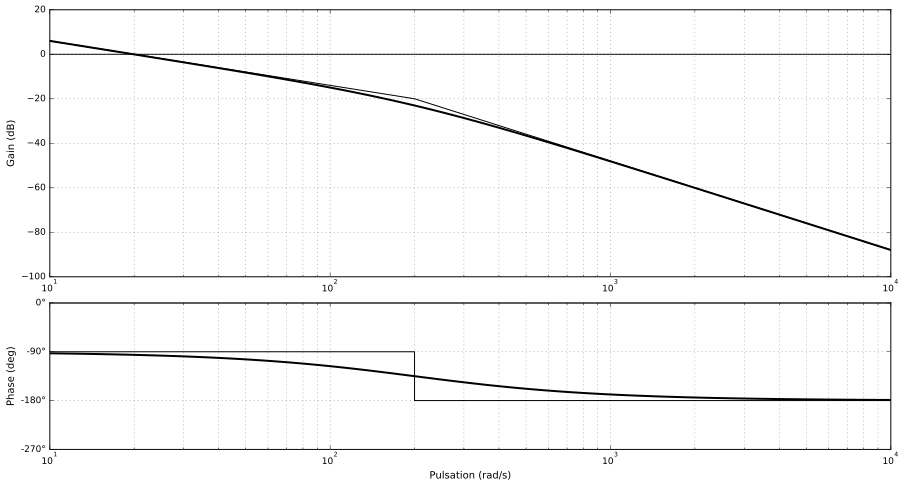
\includegraphics[width=\linewidth]{cor_01}
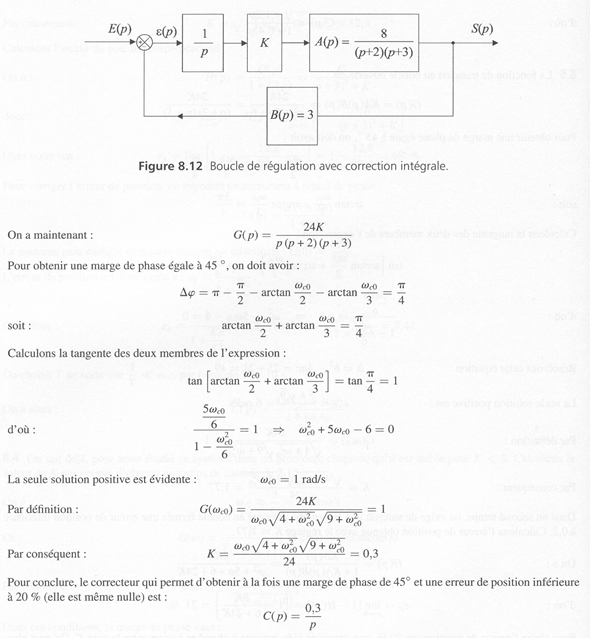
\includegraphics[width=\linewidth]{cor_02}
\end{center}


\else
\fi



%
%\subsection*{Choix d'un gain}
%
%\begin{obj}
%Déterminer le gain permettant de satisfaire le cahier des charges.
%\end{obj}
%
%\question{Déterminer graphiquement la valeur du correcteur $K$ à placer ans la chaîne directe, afin de respecter les critères de stabilité du cahier des charges.}
%
%\question{Déterminer analytiquement la valeur du correcteur $K$ à placer ans la chaîne directe, afin de respecter les critères de stabilité du cahier des charges.}
%\ifprof
%\begin{corrige}
%On a une phase de -135\degres pour $\omega=\SI{10}{rad.s^{-1}}$. Il faut donc déterminer $K$ tel que le gain soit nul en $\omega=\SI{10}{rad.s^{-1}}$.
%
%$20\log 20 - 20\log 10\sqrt{1+0,01\cdot 10^2}=20\log 20 - 20\log 10\sqrt{2}=\SI{3}{dB}$. Il faut donc diminuer le gain de \SI{3}{dB}.
%
%On cherche donc $K$ tel que $20 \log K = -3$ et il faut prendre $K=0,7$.
%\end{corrige}
%\else
%\fi
%
%\question{Quel sera alors le 1\ier dépassement pour la réponse indicielle du système ?}
%\ifprof
%\begin{corrige}
%Dépassement de 23\%.
%\end{corrige}
%\else
%\fi
%
\ifprof
\else
\end{multicols}
\fi


%\ifprof
%\else
%\noindent\begin{minipage}[c]{.4\linewidth}
%\begin{center}
%\includegraphics[width=\linewidth]{fig_03}
%\end{center}
%\end{minipage}\hfill
%\begin{minipage}[c]{.46\linewidth}
%\begin{center}
%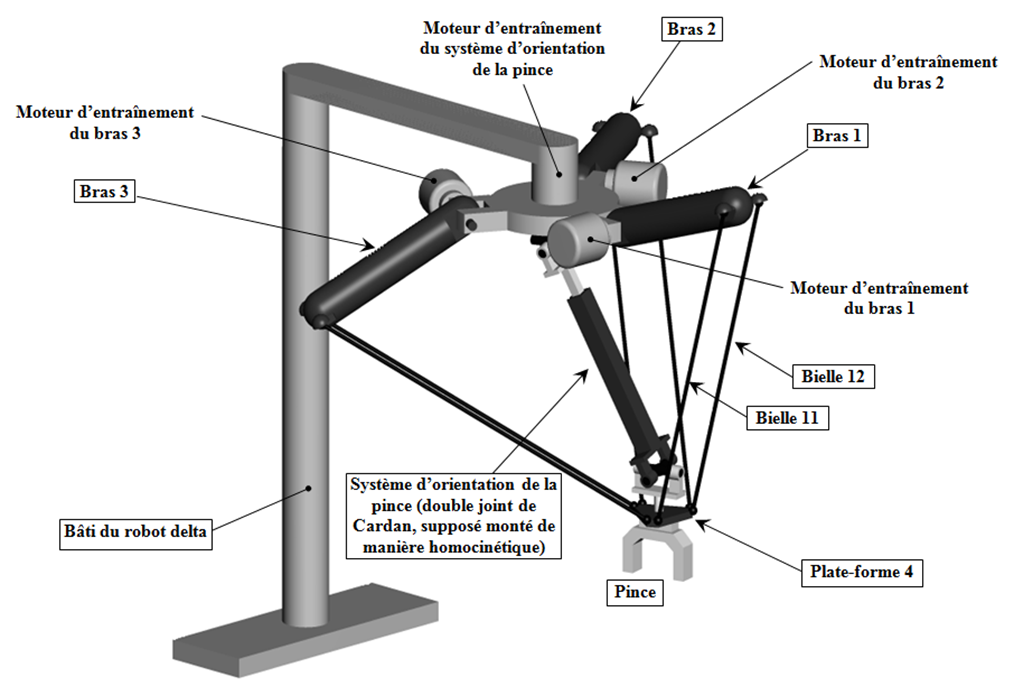
\includegraphics[width=.9\linewidth]{fig_01}
%\end{center}
%\end{minipage}

\ifprof
\else
\begin{center}
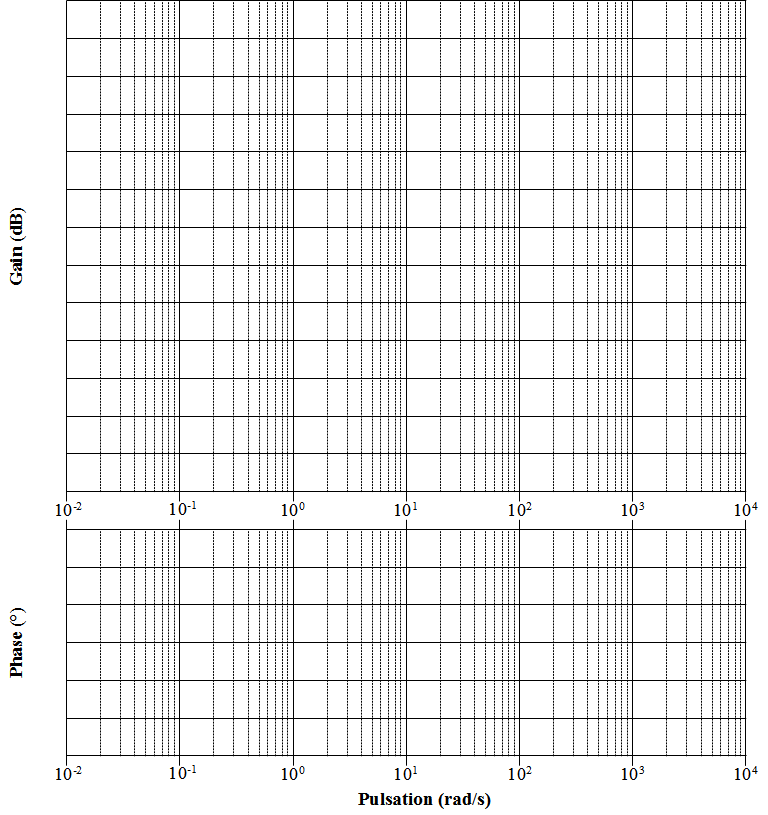
\includegraphics[width=\linewidth]{img_04}
\end{center}
\fi

%
%\begin{center}
%\includegraphics[width=\linewidth]{fig_02}
%\end{center}
%
%\begin{center}
%\includegraphics[width=\linewidth]{fig_03}
%\end{center}
%
%\begin{center}
%\includegraphics[width=.8\linewidth]{fig_04}
%\end{center}